\chapter{Radiation in Matter}
\label{ch:radiation}

Almost everything known about stars arrives as light. That light was made deep inside a star, fought its way out through layers of gas, crossed interstellar space (Chapter~\ref{ch:ism}) and finally reached a telescope. At each stage matter took some light away and added some of its own.

One equation describes all of this. It is energy conservation along a single ray (P1), with gains and losses balanced as in P4. Where the matter is thin, the equation gives emission and absorption lines. Where it is thick, it gives a blackbody and a slow, random-walk leak of energy (P5). This one equation, in its two limits, covers most of what astronomers measure.

% ==============================================================================
\section{Specific Intensity}
\label{rad:sec:intensity}

Chapter~\ref{ch:photometry} measured light by its flux, the energy crossing a unit area per unit time, which falls as the inverse square of distance (Eq.~\eqref{eq:inverse_square_flux}).

Inside a star or a cloud, light comes from every direction at once. A single flux mixes all of them together. To follow light through matter we need the light travelling in each direction separately.

Look at a white wall in an evenly lit room, first from one metre away and then from five. From farther away the wall covers less of your view, but each patch of it looks just as bright. The brightness of a surface does not fade with distance. Only its size shrinks.

The surface of the Sun is the same. Seen from Mars it covers a smaller patch of sky than seen from Earth, but each square degree of that patch is equally bright. The quantity that stays fixed along a ray is the energy per unit area, per unit time, per unit frequency and per unit solid angle, the specific intensity. Its constancy is energy conservation (P1) for a narrow bundle of rays.

The Sun in numbers. From Earth its angular radius is $0.266^\circ$. From Mars, $1.52$ times farther, it is $0.175^\circ$. The flux falls by $1.52^2=2.3$ because the solid angle falls by that factor, while the intensity of each patch is the same.

The picture is a narrow cone of rays leaving a patch of surface. Farther along, the cone is wider, but it carries the same energy in the same solid angle.

The same constancy makes the surface brightness of a galaxy independent of its distance in a static space, which is what makes it a test of the expansion of the universe. It is why gravitational lensing, which bends rays but does not create or destroy light, leaves surface brightness unchanged. Radio astronomers state it as a brightness temperature. Here it gives the intensity and the three quantities built from it.

\paragraph{Definition.} Light of frequency between $\nu$ and $\nu+d\nu$ crosses an area $dA$ in time $dt$, travelling within a solid angle $d\Omega$ about a direction that makes an angle $\theta$ with the normal of $dA$. The energy it carries defines the \textbf{specific intensity} $I_\nu$,
\begin{equation}
	dE=I_\nu\,\cos\theta\,dA\,dt\,d\nu\,d\Omega .
	\label{rad:eq:intensity_def}
\end{equation}
The factor $\cos\theta$ is the area $dA$ as seen from the direction of travel.

\paragraph{Constant along a ray.} Take two small areas $dA_1$ and $dA_2$, a distance $d$ apart in empty space, each facing the other. The light leaving $dA_1$ toward $dA_2$ is the light arriving at $dA_2$ from $dA_1$. Seen from $dA_1$, the area $dA_2$ subtends $d\Omega_1=dA_2/d^2$, and seen from $dA_2$, $dA_1$ subtends $d\Omega_2=dA_1/d^2$. Equating the two energies (P1),
\begin{align}
	I_{\nu,1}\,dA_1\,d\Omega_1
	&= I_{\nu,2}\,dA_2\,d\Omega_2 \nonumber\\
	\implies\quad I_{\nu,1}\,\frac{dA_1\,dA_2}{d^2}
	&\eqby{1} I_{\nu,2}\,\frac{dA_2\,dA_1}{d^2} \nonumber\\
	\implies\quad I_{\nu,1}
	&= I_{\nu,2} .
\end{align}
\begin{explain}
	\item The two solid angles written with the areas they subtend.
\end{explain}
\begin{equation}
	\boxed{I_\nu\ \text{is constant along a ray in empty space.}}
	\label{rad:eq:intensity_constant}
\end{equation}
The inverse-square fall of the flux is entirely the shrinking of the solid angle that a source covers.

\paragraph{Flux, energy density and pressure.} Three quantities used throughout are moments of $I_\nu$ over direction,
\begin{equation}
	F_\nu=\int I_\nu\cos\theta\,d\Omega,\qquad
	u_\nu=\frac1c\int I_\nu\,d\Omega,\qquad
	P_\nu=\frac1c\int I_\nu\cos^2\theta\,d\Omega .
	\label{rad:eq:moments}
\end{equation}
The flux $F_\nu$ is the net energy crossing a unit area. Light at speed $c$ carrying intensity $I_\nu$ through $d\Omega$ fills space with energy density $I_\nu\,d\Omega/c$, which gives $u_\nu$. Each photon carries momentum equal to its energy over $c$, and its component $\cos\theta$ across the surface, so the momentum flux, which is the pressure, is $P_\nu$. For light that is the same in every direction,
\[
F_\nu=0,\qquad u_\nu=\frac{4\pi}{c}I_\nu,\qquad P_\nu=\frac{u_\nu}{3},
\]
the same $\tfrac13$ as in the pressure integral \eqref{pr:eq:pressure_integral}, from the average of $\cos^2\theta$. With $I_\nu=B_\nu$ this is the relation $B_\nu=c\,u_\nu/4\pi$ of Eq.~\eqref{pr:eq:planck}.

A surface that sends intensity $B_\nu$ outward into every direction of the outer half-space gives the flux $F_\nu=\pi B_\nu$ (Eq.~\eqref{ph:eq:flux_pi_B}), and integrated over frequency the surface flux $\sigma_{\rm SB}T^4$ of a blackbody, Eq.~\eqref{eq:surface_flux_sb}. In the language of intensity, the factor $\pi$ is the first moment of Eq.~\eqref{rad:eq:moments} taken over the outward half of the sphere.

% ==============================================================================
\section{The Transfer Equation}
\label{rad:sec:transfer}

Chapters~\ref{ch:photometry} and~\ref{ch:ism} described extinction, in which light passing through dust is dimmed by $e^{-\tau}$ (Eq.~\eqref{ph:eq:extinction_tau}).

That is only half the story. Gas and dust also emit. A hot cloud glows, and a star's atmosphere both absorbs the light from below and adds its own.

Think of a foggy night street. A distant lamp fades as you look at it through more fog, but the fog itself glows with the light it has scattered. Through a little fog you see the lamp. Through enough fog you see only the glowing fog, and nothing about the lamp behind it.

Light travelling through matter loses a fixed fraction of itself per unit length by absorption and gains whatever the matter emits. Its intensity along the ray is a balance of the two, energy conservation (P1) with gains against losses (P4). When the matter is thick enough, the light forgets where it came from and takes on the glow of the matter.

A slab in numbers. Light of intensity $I_0$ enters a uniform slab whose own glow is $S$. If the slab has optical depth $\tau=1$, a fraction $e^{-1}=0.37$ of the entering light survives and the slab adds $0.63\,S$. At $\tau=5$ only $0.7\%$ survives and the slab adds $99.3\%$ of $S$.

The picture is Figure~\ref{rad:fig:slab}. Whatever enters, the light leaving a thick slab approaches the slab's own glow.

\begin{figure}[htbp]
	\centering
	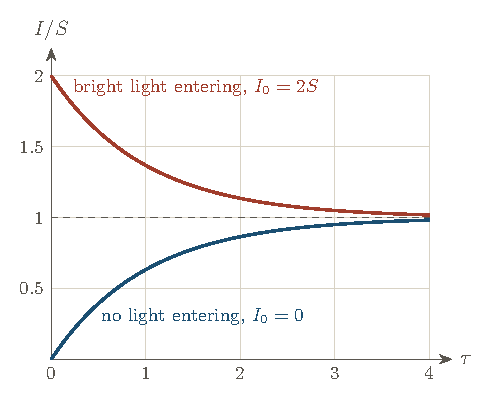
\includegraphics{fig_ch11_slab.pdf}
	\caption{The intensity leaving a uniform slab against its optical depth $\tau$, in units of the source function $S$, for entering intensity $I_0=2S$ (upper curve) and $I_0=0$ (lower curve).}
	\label{rad:fig:slab}
\end{figure}

The same equation governs radio emission from cold gas, X-rays from hot clusters, the Lyman-$\alpha$ absorption of distant quasars and the cosmic microwave background. It gives the equation and its solution.

\paragraph{The equation.} Along a path element $ds$, matter of density $\rho$ removes the fraction $\kappa_\nu\rho\,ds$ of the intensity, where $\kappa_\nu$ is the \textbf{opacity}, the absorbing area per unit mass. It also adds its own emission. Let $j_\nu$ be the energy it emits per unit volume, time, frequency and solid angle. Then (P1, P4)
\begin{equation}
	\boxed{\dv{I_\nu}{s}=-\kappa_\nu\rho\,I_\nu+j_\nu .}
	\label{rad:eq:transfer}
\end{equation}
Scattering removes light from a ray just as absorption does, so it counts in $\kappa_\nu$, and the light it sends into the ray counts in $j_\nu$.

\paragraph{Optical depth and source function.} Two combinations make the equation simpler. The \textbf{optical depth} along the ray, $d\tau_\nu=\kappa_\nu\rho\,ds$, is the path length counted in mean free paths $1/(\kappa_\nu\rho)$, the same $\tau$ as in Chapter~\ref{ch:photometry}. The \textbf{source function} $S_\nu=j_\nu/(\kappa_\nu\rho)$ is the ratio of emission to absorption. Dividing Eq.~\eqref{rad:eq:transfer} by $\kappa_\nu\rho$,
\begin{equation}
	\dv{I_\nu}{\tau_\nu}=-I_\nu+S_\nu .
	\label{rad:eq:transfer_tau}
\end{equation}
The intensity always moves toward the source function. If $I_\nu>S_\nu$ it falls, and if $I_\nu<S_\nu$ it rises.

\paragraph{Formal solution.} Multiply Eq.~\eqref{rad:eq:transfer_tau} by $e^{\tau_\nu}$ and integrate from $0$, where the ray enters with $I_\nu(0)$, to $\tau_\nu$,
\begin{align}
	\dv{\tau_\nu}\Big(I_\nu\,e^{\tau_\nu}\Big)
	&\eqby{1} S_\nu\,e^{\tau_\nu} \nonumber\\
	\implies\quad I_\nu(\tau_\nu)
	&\eqby{2} I_\nu(0)\,e^{-\tau_\nu}+\int_0^{\tau_\nu}S_\nu(\tau')\,e^{-(\tau_\nu-\tau')}\,d\tau' .
\end{align}
\begin{explain}
	\item The product rule. The terms in $I_\nu$ combine into a total derivative.
	\item Integrate, then divide by $e^{\tau_\nu}$.
\end{explain}
The entering light is dimmed by $e^{-\tau_\nu}$. Each layer adds its emission, dimmed by the matter between it and the end of the ray. For a uniform slab, $S_\nu$ is constant and
\begin{equation}
	\boxed{I_\nu=I_\nu(0)\,e^{-\tau_\nu}+S_\nu\big(1-e^{-\tau_\nu}\big).}
	\label{rad:eq:slab}
\end{equation}
Two limits follow, chosen by the ratio of the size of the slab to the mean free path (P6).
\begin{itemize}
	\item \textbf{Optically thin}, $\tau_\nu\ll1$. Then $I_\nu\approx I_\nu(0)+S_\nu\tau_\nu$. The slab adds emission in proportion to the amount of matter. Where $\kappa_\nu$ is large, at the frequency of a line, the emission is large, so a thin glowing gas shows emission lines.
	\item \textbf{Optically thick}, $\tau_\nu\gg1$. Then $I_\nu\to S_\nu$, whatever entered. We see only the last mean free path or so of the matter.
\end{itemize}
With no emission, $S_\nu=0$, this is the extinction law of Eq.~\eqref{ph:eq:flux_tau}.

% ==============================================================================
\section{Kirchhoff's Law and Local Thermodynamic Equilibrium}
\label{rad:sec:kirchhoff}

The Planck spectrum was derived by counting the states of light (Eq.~\eqref{pr:eq:planck}), and Chapter~\ref{ch:photometry} treated stars as blackbodies.

A star is not a closed box at one temperature. Its temperature falls outward and light escapes. It is not obvious why its light should look like a blackbody, or why its spectrum should have dark lines.

Look into a furnace. A poker left in the coals glows with exactly the colour of the coals around it, and its outline nearly disappears. Everything in the furnace glows alike, whatever it is made of. A material that absorbs well also glows well, in just the right proportion, because otherwise the poker would end up hotter or colder than the coals.

The same rule holds for each small parcel of a star. Matter that absorbs strongly at some frequency also emits strongly there, and the ratio of the two is fixed by its temperature. This is detailed balance (P4) for absorption and emission, with the counted spectrum of light (P3).

Two layers in numbers. Suppose the continuum at $500\,\mathrm{nm}$ reaches us from a layer at $6000\,\mathrm K$, and the centre of a strong line from a higher layer at $4500\,\mathrm K$. The intensity at line centre is then $B_\nu(4500\,\mathrm K)/B_\nu(6000\,\mathrm K)=0.20$ of the continuum. The line is dark.

The picture is two depths in an atmosphere. At most frequencies we see down to a deep, hot layer. At the frequency of a line the gas is more opaque, so we see only a high, cooler layer.

The same law gives the dark Fraunhofer lines of the Sun, the bright lines of glowing nebulae, the darkening of the Sun's edge, and the nearly perfect blackbody of the microwave background. It gives the source function of matter in equilibrium and the way lines form.

\paragraph{Kirchhoff's law.} Inside a closed cavity in full thermodynamic equilibrium at temperature $T$, the light is the same everywhere and in every direction, and by P3 it is Planck light, $I_\nu=B_\nu(T)$. Nothing changes along a ray, so Eq.~\eqref{rad:eq:transfer} gives
\begin{align}
	0
	&\eqby{1} -\kappa_\nu\rho\,B_\nu(T)+j_\nu \nonumber\\
	\implies\quad S_\nu
	&\eqby{2} \frac{j_\nu}{\kappa_\nu\rho}=B_\nu(T) .
\end{align}
\begin{explain}
	\item $\dv*{I_\nu}{s}=0$ with $I_\nu=B_\nu$. Every process is balanced by its reverse (P4).
	\item The definition of $S_\nu$.
\end{explain}
\begin{equation}
	\boxed{j_\nu=\kappa_\nu\rho\,B_\nu(T).}
	\label{rad:eq:kirchhoff}
\end{equation}
Emission and absorption are tied together by the Planck function of the matter's temperature.

\paragraph{Local thermodynamic equilibrium.} The emission and absorption of a parcel depend on the parcel itself, on its atoms and how they are excited, not on the light passing through. Where collisions keep each parcel close to equilibrium inside itself, the local thermodynamic equilibrium of Section~\ref{sg:sec:rotation}, its atoms are excited as in equilibrium at the local temperature. Eq.~\eqref{rad:eq:kirchhoff} then holds point by point, even though the light passing through is not Planck light,
\begin{equation}
	S_\nu=B_\nu\big(T(\vecr)\big)\qquad\text{(local thermodynamic equilibrium).}
	\label{rad:eq:lte_source}
\end{equation}
A thick layer at one temperature then emits Planck light, as a blackbody does, without being a closed box.

\paragraph{Absorption lines.} In an atmosphere the temperature falls outward. By Eq.~\eqref{rad:eq:slab} we see light from about one mean free path deep, $\tau_\nu\approx1$ along our line of sight (more exactly $\tau_\nu\approx\tfrac23$, Section~\ref{rad:sec:grey}). At the frequency of a line, $\kappa_\nu$ is large, so $\tau_\nu=1$ is reached higher up, where the gas is cooler and $B_\nu$ is smaller. The line is darker than the continuum on either side. If the temperature rose outward, as it does in the solar chromosphere, the same argument would give emission lines. The edge of the Sun looks darker than its centre for the same reason. Looking at the edge, the line of sight runs slantwise and reaches $\tau=1$ in higher, cooler layers.

% ==============================================================================
\section{Diffusion of Light}
\label{rad:sec:diffusion}

Deep inside a star the optical depth to the surface is enormous, and by the thick limit of Eq.~\eqref{rad:eq:slab} the light at each point is nearly Planck light at the local temperature.

If the light were exactly Planck light, the same in every direction, it would carry no net flux (Section~\ref{rad:sec:intensity}). But the Sun does shine. A small departure from equal light in all directions must carry its whole luminosity outward.

Think again of perfume in still air (Problem~\ref{pr:prob:perfume}). Each molecule wanders at random, but a little more perfume drifts away from the bottle than toward it, because there is more perfume near the bottle. A net flow appears with no push in any direction, only a gradient.

Photons in a star do the same. Each is absorbed and re-emitted after a short free path, in a random direction. There is slightly more light where the gas is hotter, so a little more light drifts outward than inward. This is a random walk (P5), with the energy density of light $aT^4$ in place of the number of perfume molecules.

The Sun in numbers. Near its centre a photon's free path is of order a millimetre to a centimetre. To random-walk out across a radius of $7\times10^8\,\mathrm m$ takes $R^2/(sc)$, Eq.~\eqref{pr:eq:walk_time}, which is $5\times10^3$ years for $s=1\,\mathrm{cm}$ and $5\times10^4$ years for $s=1\,\mathrm{mm}$. A straight flight would take $2.3$ seconds.

The picture is the random walk of Figure~\ref{pr:fig:random_walk}, with photons in place of walkers, drifting slowly down the slope of temperature.

The same diffusion carries heat through the interiors of stars, carries neutrinos out of a collapsing stellar core, and smooths the early universe on small scales before atoms form. It gives the flux of light deep inside a star, by two routes.

\paragraph{Route A, the random walk.} The diffusion flux of Eq.~\eqref{pr:eq:fick} applies to anything that walks at random. For light, the walkers are photons and the quantity that flows is energy. With energy density $aT^4$ (Eq.~\eqref{pr:eq:photon_gas}) in place of $n$, speed $c$, and step length $1/(\kappa\rho)$,
\begin{equation}
	F=-\frac13\,c\,\frac{1}{\kappa\rho}\,\dv{(aT^4)}{r}=-\frac{c}{3\kappa\rho}\,\dv{(aT^4)}{r}.
	\label{rad:eq:diffusion_flux}
\end{equation}

\paragraph{Route B, the momentum of light.} Multiply the transfer equation \eqref{rad:eq:transfer} by $\cos\theta/c$ and integrate over all directions. Along a radial coordinate, $\dv*{}{s}=\cos\theta\,\dv*{}{r}$ for the part of the change that matters deep inside a star, where curvature over one free path is negligible. Then
\begin{align}
	\dv{r}\,\frac1c\int I_\nu\cos^2\theta\,d\Omega
	&\eqby{1} -\frac{\kappa_\nu\rho}{c}\int I_\nu\cos\theta\,d\Omega+\frac{j_\nu}{c}\int\cos\theta\,d\Omega \nonumber\\
	\implies\quad \dv{P_\nu}{r}
	&\eqby{2} -\frac{\kappa_\nu\rho}{c}\,F_\nu .
\end{align}
\begin{explain}
	\item Eq.~\eqref{rad:eq:transfer} with $\dv*{}{s}=\cos\theta\,\dv*{}{r}$, times $\cos\theta/c$, integrated over $d\Omega$.
	\item The moments of Eq.~\eqref{rad:eq:moments}. Emission is the same in all directions, so $\int\cos\theta\,d\Omega=0$ removes it.
\end{explain}
This is momentum conservation (P1) for light. The gradient of the pressure of light equals the momentum per unit volume and time that the light gives to the matter. Deep inside, $P=aT^4/3$, and with $\kappa$ a suitable average over frequency,
\begin{equation}
	\dv{r}\left(\frac{aT^4}{3}\right)=-\frac{\kappa\rho}{c}\,F,
\end{equation}
which is Eq.~\eqref{rad:eq:diffusion_flux} again. (The right average weights $1/\kappa_\nu$ by $\partial B_\nu/\partial T$, so the frequencies where matter is most transparent carry most of the flux. It is called the Rosseland mean.)

\paragraph{The transport equation.} Write $F=L(r)/(4\pi r^2)$, where $L(r)$ is the luminosity through the sphere of radius $r$, and $\dv*{(aT^4)}{r}=4aT^3\,\dv*{T}{r}$. Then
\begin{equation}
	\boxed{\dv{T}{r}=-\frac{3\,\kappa\rho\,L(r)}{16\pi a c\,r^2T^3}.}
	\label{rad:eq:radiative_transport}
\end{equation}
The temperature gradient needed to carry a luminosity grows with the opacity. Opaque matter needs a steep fall of temperature to push the same energy through. This is the radiative transport equation of a star (Section~\ref{st:sec:four_equations}).

% ==============================================================================
\section{The Eddington Luminosity}
\label{rad:sec:eddington}

The light flowing out of a star pushes on the matter it passes through, with the force found in Route B above.

The brighter a star, the harder its light pushes. At some brightness the push must match gravity.

Think of standing in a strong wind. A breeze does nothing, a gale pushes you over. Somewhere between, the push of the wind equals the grip your weight gives you on the ground.

The matter at the surface of a star is held down by gravity and pushed out by the momentum of the light streaming past it (P1 for light, P2 for gravity). Both forces fall off as $1/r^2$, so their ratio depends only on the luminosity and the mass. Above a certain luminosity, the Eddington luminosity, no star can hold on to its outer layers.

The Sun in numbers. For ionised hydrogen, where light is scattered by free electrons, the limit is $1.3\times10^{31}\,\mathrm W$, about $3.3\times10^4$ times the Sun's luminosity. The Sun is far below it.

The picture is a parcel of gas with gravity pulling it inward and a stream of photons pushing it outward. The ratio of the two arrows does not depend on the radius.

The same limit caps the luminosity of the most massive stars, and it caps how fast black holes can swallow gas, since infalling gas radiates and the light pushes back. A quasar shining at $10^{39}\,\mathrm W$ must hold at least $10^8$ solar masses. It gives the maximum luminosity of a body of mass $M$.

\paragraph{The limit.} From Route B, light of flux $F$ gives the matter a force per unit volume $\kappa\rho F/c$, so a force per unit mass $\kappa F/c$. Gravity pulls with $GM/r^2$ per unit mass. With $F=L/(4\pi r^2)$ the two balance when
\begin{align}
	\frac{\kappa}{c}\,\frac{L}{4\pi r^2}
	&= \frac{GM}{r^2} \nonumber\\
	\implies\quad L
	&= \frac{4\pi GMc}{\kappa} .
\end{align}
\begin{equation}
	\boxed{L_{\rm Edd}=\frac{4\pi GMc}{\kappa}.}
	\label{rad:eq:eddington}
\end{equation}
The radius has dropped out. In hot ionised gas the opacity is scattering by free electrons, with the Thomson cross-section $\sigma_T$ of Eq.~\eqref{eq:thomson_cross_section} per electron. For pure hydrogen there is one electron per mass $m_{\rm H}$, so $\kappa=\sigma_T/m_{\rm H}=0.040\,\mathrm{m^2\,kg^{-1}}$ and
\[
L_{\rm Edd}=1.3\times10^{31}\,\mathrm W\left(\frac{M}{M_\odot}\right)=3.3\times10^4\,L_\odot\left(\frac{M}{M_\odot}\right).
\]
Any larger opacity lowers the limit.

% ==============================================================================
\section{Einstein Coefficients}
\label{rad:sec:lines}

Kirchhoff's law fixed the ratio of emission to absorption for matter in local thermodynamic equilibrium (Eq.~\eqref{rad:eq:kirchhoff}).

It did not say what an atom actually does, or what happens when collisions are too rare to keep its levels in equilibrium, as in thin interstellar gas.

Think of a ball resting at the bottom of a step. A kick can lift it onto the step, and from the step it can roll back down by itself. A kick can also knock it down sooner than it would have rolled. If the ball spends time on and off the step in the proportions the temperature demands, the three kinds of move must be related.

An atom with two levels makes three kinds of transition. Light can lift it, it can drop by itself, and light can push it down sooner (stimulated emission). Detailed balance (P4) with Planck light and Boltzmann populations (P3) fixes how the three rates are related. Since the rates belong to the atom alone, the relations hold everywhere, in equilibrium or not.

The $21\,\mathrm{cm}$ line in numbers. The upper level of hydrogen's ground state drops by itself at the rate $2.9\times10^{-15}\,\mathrm{s^{-1}}$ (Eq.~\eqref{is:eq:A21}), once in $11$ million years. In interstellar gas, collisions change the level far more often than that, so the populations follow the gas temperature (Section~\ref{sec:ism_hydrogen}).

The picture is two levels with three arrows between them, one up and two down.

The same relations give the strength of every spectral line, the gain of lasers and of the masers seen in star-forming clouds, and the condition for a line to form out of equilibrium. They give the three coefficients and the relations between them.

\paragraph{Three rates.} Let level 1 (lower) and level 2 (upper) be single states separated by $h\nu$. In light of energy density $u_\nu$ at the line frequency,
\begin{itemize}
	\item absorption lifts an atom from 1 to 2 at the rate $B_{12}\,u_\nu$ per atom,
	\item spontaneous emission drops it from 2 to 1 at the rate $A_{21}$ per atom,
	\item stimulated emission drops it from 2 to 1 at the rate $B_{21}\,u_\nu$ per atom.
\end{itemize}
These are the \textbf{Einstein coefficients}. They belong to the atom.

\paragraph{Relations.} In thermodynamic equilibrium at temperature $T$, the upward and downward flows balance (P4), the populations follow the Boltzmann factor, $N_2/N_1=e^{-h\nu/k_BT}$, and the light is Planck light (P3),
\begin{align}
	N_1B_{12}\,u_\nu
	&\eqby{1} N_2\big(A_{21}+B_{21}\,u_\nu\big) \nonumber\\
	\implies\quad u_\nu
	&\eqby{2} \frac{A_{21}}{B_{12}\,e^{h\nu/k_BT}-B_{21}} .
\end{align}
\begin{explain}
	\item Detailed balance between level 1 and level 2.
	\item Solve for $u_\nu$ and use $N_1/N_2=e^{h\nu/k_BT}$.
\end{explain}
This must equal the Planck energy density, $u_\nu=(8\pi h\nu^3/c^3)/(e^{h\nu/k_BT}-1)$ from Section~\ref{pr:sec:p3}, at every temperature. That is possible only if
\begin{equation}
	\boxed{B_{12}=B_{21},\qquad A_{21}=\frac{8\pi h\nu^3}{c^3}\,B_{21}.}
	\label{rad:eq:einstein}
\end{equation}
One coefficient fixes the other two. The relations hold for the atom in any surroundings, since the coefficients do not depend on whether the gas is in equilibrium. Stimulated emission is required by them. Without it no choice of coefficients could reproduce the Planck spectrum. (For levels with several states, each $B$ is multiplied by the number of states of its starting level.)

\paragraph{When local equilibrium fails.} The populations follow the gas temperature when collisions move atoms between the levels much faster than spontaneous emission does. The ratio of the collision rate to $A_{21}$ decides (P6). In dense stellar atmospheres collisions win, and local thermodynamic equilibrium holds. In thin nebulae, light and spontaneous decay set the populations instead, and lines must be computed from the rates themselves. If some process fills the upper level faster than the lower one, $N_2>N_1$, the net absorption $(N_1-N_2)B_{12}u_\nu$ turns negative and the gas amplifies light passing through it. Such masers are seen in water and hydroxyl molecules in star-forming clouds.

% ==============================================================================
\section{The Grey Atmosphere}
\label{rad:sec:grey}

The effective temperature was defined in Chapter~\ref{ch:photometry} by $L=4\pi R^2\sigma_{\rm SB}T_{\rm eff}^4$ (Eq.~\eqref{eq:stefan_boltzmann_luminosity}), as if the star had one surface at one temperature.

A star has no sharp surface. Its temperature falls continuously outward, and the light we see comes from a range of depths. Where is the effective temperature actually found?

Think of looking into a pool of murky water. You see down to some depth where the water stops being clear, and no farther. The bottom you see is not a surface in the water but the depth at which the murk has added up to enough.

A star's photosphere is such a depth. It lies at a fixed optical depth, and the temperature there is the effective temperature. The calculation uses momentum conservation for light (P1), the steady flow of energy through the atmosphere (P4), and Planck light at the local temperature (P3).

In numbers, the result below puts the effective temperature at an optical depth of $\tfrac23$, and the topmost gas, at $\tau=0$, at $2^{-1/4}=0.84$ of it. For the Sun that is $4850\,\mathrm K$ at the top against $5772\,\mathrm K$ at the photosphere.

The picture is Figure~\ref{rad:fig:grey}, a temperature that rises slowly with depth through the layers we see.

\begin{figure}[htbp]
	\centering
	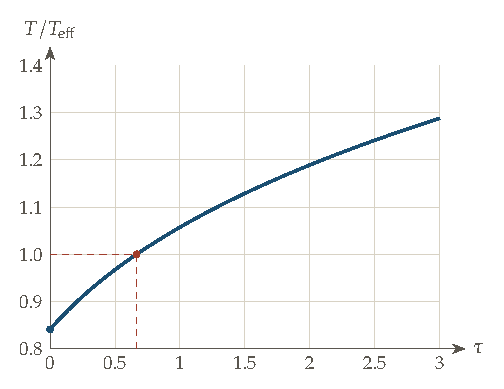
\includegraphics{fig_ch11_grey_atmosphere.pdf}
	\caption{The temperature of a grey atmosphere against optical depth, in units of the effective temperature. The point at $\tau=\tfrac23$ marks $T=T_{\rm eff}$, and the point at $\tau=0$ marks $T=2^{-1/4}T_{\rm eff}$.}
	\label{rad:fig:grey}
\end{figure}

The same calculation, with the opacity's dependence on frequency added, is the starting point of every model stellar atmosphere, and of planetary atmospheres warmed from below. It gives the temperature through the atmosphere.

\paragraph{Assumptions.} Take the opacity the same at all frequencies (grey), so frequency can be integrated out. Measure the optical depth $\tau$ inward from the top. The atmosphere is thin compared with the star, so it is treated as flat, and no energy is made in it, so the flux $F$ is the same at every depth (P1, P4).

\paragraph{Temperature against depth.} The momentum equation of Route B, with $d\tau=-\kappa\rho\,dr$, reads $\dv*{P_{\rm light}}{\tau}=F/c$. With $F$ constant,
\begin{equation}
	P_{\rm light}(\tau)=\frac Fc\,\tau+P_{\rm light}(0).
\end{equation}
Two approximations close it. Deep down the light is nearly the same in all directions, so $P_{\rm light}=u/3$, and Eddington took this to hold at all depths. At the top, light only leaves and none comes in. If the outgoing light is spread evenly over the outer half of directions with intensity $I^+$, then $F=\pi I^+$ and $u=2\pi I^+/c$ from Eq.~\eqref{rad:eq:moments}, so $u(0)=2F/c$. Then
\begin{align}
	\frac{u}{3}
	&\eqby{1} \frac Fc\,\tau+\frac{2F}{3c} \nonumber\\
	\implies\quad aT^4
	&\eqby{2} \frac{3F}{c}\left(\tau+\frac23\right) \nonumber\\
	&\eqby{3} \frac34\,aT_{\rm eff}^4\left(\tau+\frac23\right).
\end{align}
\begin{explain}
	\item $P_{\rm light}=u/3$ at all depths and $P_{\rm light}(0)=u(0)/3=2F/(3c)$.
	\item Local thermodynamic equilibrium, $u=aT^4$.
	\item $F=\sigma_{\rm SB}T_{\rm eff}^4$ and $\sigma_{\rm SB}=ac/4$ (Section~\ref{pr:sec:p3}).
\end{explain}
\begin{equation}
	\boxed{T^4=\frac34\,T_{\rm eff}^4\left(\tau+\frac23\right).}
	\label{rad:eq:grey}
\end{equation}
The temperature equals $T_{\rm eff}$ at $\tau=\tfrac23$. That depth is the \textbf{photosphere}, the layer the effective temperature describes. Above it the temperature levels off at $2^{-1/4}T_{\rm eff}$, and below it the temperature keeps rising, as $\tau^{1/4}$ deep down, where the diffusion of Section~\ref{rad:sec:diffusion} takes over.

% ==============================================================================
\section{Problem Set: Radiation in Matter}

\subsection{Problem 1: The Sun Seen From Mars}
\label{rad:prob:mars}

\textbf{Problem Statement}: Mars is $1.52$ times farther from the Sun than the Earth. Compare (a) the flux of sunlight and (b) the specific intensity of the solar disk seen from the two planets. (c) Why does a camera on Mars need a longer exposure for a picture of the whole landscape, but not for a picture of the Sun's disk filling the same number of pixels?

\textbf{Essential Ideas}:
\begin{itemize}
	\item The flux falls as $1/d^2$ (Eq.~\eqref{eq:inverse_square_flux}).
	\item The intensity is constant along a ray (Eq.~\eqref{rad:eq:intensity_constant}).
\end{itemize}

\textbf{Detailed Solutions}:
\begin{enumerate}[label=(\alph*)]
	\item \textbf{Flux}. $F_{\rm Mars}/F_\oplus=1/1.52^2$.
	\[
	\boxed{F_{\rm Mars}=0.43\,F_\oplus.}
	\]
	\item \textbf{Intensity}. Unchanged.
	\[
	\boxed{I_{\rm Mars}=I_\oplus.}
	\]
	\item \textbf{Exposures}. A landscape is lit by the total flux, which is lower on Mars. A pixel looking at the Sun's disk collects intensity times the solid angle of one pixel, and both are the same.
\end{enumerate}

\subsection{Problem 2: How Opaque Is a Dark Cloud?}
\label{rad:prob:cloud}

\textbf{Problem Statement}: A dark cloud dims background starlight in the visual band by $A_V=10$ magnitudes, and the cloud's own glow in that band is negligible. (a) What is its optical depth? (b) What fraction of the starlight gets through? (c) At $2.2\,\mu\mathrm m$ the extinction is about $0.11$ of the visual value. What fraction gets through there?

\textbf{Essential Ideas}:
\begin{itemize}
	\item With $S_\nu=0$, Eq.~\eqref{rad:eq:slab} gives $I=I_0e^{-\tau}$, and $A=2.5\log_{10}(I_0/I)=1.086\,\tau$ (Eq.~\eqref{ph:eq:extinction_tau}).
\end{itemize}

\textbf{Detailed Solutions}:
\begin{enumerate}[label=(\alph*)]
	\item \textbf{Optical depth}. $\tau_V=10/1.086$.
	\[
	\boxed{\tau_V\simeq9.2.}
	\]
	\item \textbf{Visual transmission}. $e^{-9.2}$.
	\[
	\boxed{I/I_0\simeq1.0\times10^{-4}.}
	\]
	\item \textbf{Infrared}. $\tau=0.11\times9.2=1.0$, so $e^{-1.0}=0.36$.
	\[
	\boxed{I/I_0\simeq0.36.}
	\]
	The cloud is opaque in visible light and nearly transparent in the near infrared, which is why young stars inside such clouds are found with infrared telescopes.
\end{enumerate}

\subsection{Problem 3: How Long Light Takes to Leave the Sun}
\label{rad:prob:escape}

\textbf{Problem Statement}: Take the mean free path of a photon inside the Sun to be $s=1\,\mathrm{mm}$ throughout. Estimate the time for energy made at the centre to random-walk to the surface, $R_\odot=6.96\times10^8\,\mathrm m$. How many free paths is that?

\textbf{Essential Ideas}:
\begin{itemize}
	\item The random-walk time $R^2/(sc)$, Eq.~\eqref{pr:eq:walk_time}, and $N=(R/s)^2$ steps.
\end{itemize}

\textbf{Detailed Solutions}:
\[
\boxed{t=\frac{(6.96\times10^8)^2}{10^{-3}\times3.00\times10^8}\,\mathrm s\simeq1.6\times10^{12}\,\mathrm s\simeq5\times10^4\ \text{years},\qquad N\simeq5\times10^{23}.}
\]
The light we see today left the core tens of thousands of years ago, as energy. The individual photons were absorbed and re-emitted along the way, about $5\times10^{23}$ times.

\subsection{Problem 4: Eddington Limits}
\label{rad:prob:eddington}

\textbf{Problem Statement}: Using electron scattering in ionised hydrogen, $\kappa=0.040\,\mathrm{m^2\,kg^{-1}}$, find the Eddington luminosity of (a) a star of $100\,M_\odot$ and (b) a black hole of $10^8\,M_\odot$. (c) A quasar emits $10^{40}\,\mathrm W$. What is the least mass that can power it?

\textbf{Essential Ideas}:
\begin{itemize}
	\item $L_{\rm Edd}=4\pi GMc/\kappa=1.3\times10^{31}\,\mathrm W\,(M/M_\odot)$, Eq.~\eqref{rad:eq:eddington}.
\end{itemize}

\textbf{Detailed Solutions}:
\begin{enumerate}[label=(\alph*)]
	\item \textbf{Massive star}.
	\[
	\boxed{L_{\rm Edd}\simeq1.3\times10^{33}\,\mathrm W\simeq3\times10^6\,L_\odot.}
	\]
	The most massive stars shine at a good fraction of this, so they lose mass in strong winds.
	\item \textbf{Black hole}.
	\[
	\boxed{L_{\rm Edd}\simeq1.3\times10^{39}\,\mathrm W.}
	\]
	\item \textbf{Quasar}. $M\ge L\kappa/(4\pi Gc)=10^{40}/(1.3\times10^{31})\,M_\odot$.
	\[
	\boxed{M\gtrsim8\times10^8\,M_\odot.}
	\]
\end{enumerate}

\subsection{Problem 5: The Surface of a Grey Star}
\label{rad:prob:grey}

\textbf{Problem Statement}: In the grey atmosphere of Eq.~\eqref{rad:eq:grey} for a star with $T_{\rm eff}=5772\,\mathrm K$, find the temperature (a) at the top, (b) at $\tau=\tfrac23$, and (c) at $\tau=10$.

\textbf{Essential Ideas}:
\begin{itemize}
	\item $T=T_{\rm eff}\,[\tfrac34(\tau+\tfrac23)]^{1/4}$.
\end{itemize}

\textbf{Detailed Solutions}:
\begin{enumerate}[label=(\alph*)]
	\item \textbf{Top}. $T=2^{-1/4}T_{\rm eff}$.
	\[
	\boxed{T(0)\simeq4850\,\mathrm K.}
	\]
	\item \textbf{Photosphere}.
	\[
	\boxed{T(\tfrac23)=T_{\rm eff}=5772\,\mathrm K.}
	\]
	\item \textbf{Deeper}. $[\tfrac34\times10.67]^{1/4}=1.68$.
	\[
	\boxed{T(10)\simeq9700\,\mathrm K.}
	\]
\end{enumerate}
